\documentclass[10pt,leqno]{article}
\usepackage[T1]{fontenc}
\usepackage[utf8]{inputenc}
\usepackage{lmodern}
\usepackage{amsmath,amssymb,mathtools}
\usepackage{mathrsfs}
\usepackage{tikz-cd}
\usepackage{geometry}
\usepackage{enumitem}
\geometry{margin=0.86in}
\setlength{\parindent}{1.2em}
\setlength{\parskip}{0.12em}
\emergencystretch=3em
\setlist{leftmargin=2.1em,itemsep=0.08em,topsep=0.2em}
\newcommand{\A}{\mathbb{A}}
\newcommand{\C}{\mathbb{C}}
\newcommand{\F}{\mathbb{F}}
\newcommand{\Q}{\mathbb{Q}}
\newcommand{\R}{\mathbb{R}}
\newcommand{\Z}{\mathbb{Z}}
\newcommand{\Gm}{\mathbb{G}_m}
\newcommand{\Ql}{\mathbb{Q}_\ell}
\newcommand{\Fp}{\mathbb{F}_q}
\newcommand{\Fpb}{\overline{\mathbb{F}}_q}
\newcommand{\Gal}{\operatorname{Gal}}
\newcommand{\Pic}{\operatorname{Pic}}
\newcommand{\Spec}{\operatorname{Spec}}
\newcommand{\Lie}{\operatorname{Lie}}
\newcommand{\End}{\operatorname{End}}
\newcommand{\Hom}{\operatorname{Hom}}
\newcommand{\GL}{\operatorname{GL}}
\newcommand{\SO}{\operatorname{SO}}
\newcommand{\Spin}{\operatorname{Spin}}
\newcommand{\CSpin}{\operatorname{CSpin}}
\newcommand{\Ker}{\operatorname{Ker}}
\newcommand{\LieJ}{\operatorname{Lie}}
\newcommand{\ad}{\operatorname{ad}}
\newcommand{\tr}{\operatorname{tr}}
\newcommand{\dfn}{\mathrm{dfn}}
\newcommand{\id}{\operatorname{id}}
\newcommand{\iso}{\xrightarrow{\sim}}
\newcommand{\onto}{\twoheadrightarrow}
\newcommand{\into}{\hookrightarrow}
\newcommand{\Cl}{\operatorname{C}}
\renewcommand{\thefootnote}{\fnsymbol{footnote}}

\providecommand{\Aut}{\operatorname{Aut}}
\providecommand{\Sp}{\operatorname{Sp}}
\providecommand{\NS}{\operatorname{NS}}
\providecommand{\Mat}{\operatorname{M}}
\providecommand{\Gr}{\operatorname{Gr}}
\providecommand{\pr}{\operatorname{pr}}
\providecommand{\Tr}{\operatorname{Tr}}
\providecommand{\rk}{\operatorname{rk}}
\providecommand{\codim}{\operatorname{codim}}
\providecommand{\Inv}{\operatorname{Inv}}

\begin{document}

\begin{center}
{\large Inventiones math. 15, 206--226 (1972)}\\
{\small \copyright{} by Springer-Verlag 1972}\\[3.0em]
{\Large\bfseries The Weil Conjecture for K3 Surfaces}\\[1.5em]
{Pierre Deligne\textsuperscript{*} (Bures-sur-Yvette)}
\end{center}

\section*{1. Statement of the Theorem}

Let $\Fp$ be a field with $q$ elements, let $\overline{\F}_q$ be an algebraic closure of $\Fp$, let $\varphi\in\Gal(\overline{\F}_q/\Fp)$ be the Frobenius substitution $x\mapsto x^q$, and let $F=\varphi^{-1}$ be the ``geometric Frobenius.''

Let $X$ be a scheme (separated and of finite type) over $\Fp$, and let $\overline X$ be the scheme over $\overline{\F}_q$ obtained from it by extension of scalars. For every closed point $x$ of $X$, let $\deg(x)=[k(x):\Fp]$ be the degree of the residue-field extension over $\Fp$. The zeta function $Z(X,t)\in\Z[[t]]$ is defined by
\[
Z(X,t)=\prod_{x\in X}(1-t^{\deg(x)})^{-1}\qquad(x\text{ a closed point of }X),
\]
\[
\log Z(X,t)=\sum_{n>0}\#X(\F_{q^n})\frac{t^n}{n}.
\]

For every prime number $\ell$ prime to $q$, the $\ell$-adic cohomology with proper supports $H_c^i(\overline X,\Ql)$ of $\overline X$ is a finite-dimensional vector space over $\Ql$, on which $\Gal(\overline{\F}_q/\Fp)$ acts by transport of structure. By Grothendieck, one has
\[
Z(X,t)=\prod_i\det(1-Ft,H_c^i(\overline X,\Ql))^{(-1)^{i+1}}.
\]

Take $X$ to be a nonsingular projective surface. In this case it is known that the factors
\[
P_i(t)=\det(1-Ft,H^i(\overline X,\Ql))
\]
of $Z(X,t)$ are polynomials with integer coefficients independent of $\ell$. The Weil conjecture asserts here that the roots of $P_i(t)$ have complex absolute value $q^{-i/2}$. This conjecture is invariant under finite extension of the finite base field. For $X$ as above, and $i\ne2$, it follows from Weil [9]. If, for simplicity, $X$ is assumed geometrically connected, one indeed has
\[
P_0(t)=1-t,
\qquad
P_4(t)=1-q^2t,
\]
\[
P_1(t)=\det(1-\varphi t;T_\ell(\Pic^0(X)_{\mathrm{red}})),
\qquad
P_3(t)=P_1(qt).
\]
\footnotetext[1]{This article was written during a stay at the University of Warwick, which I thank for its hospitality.}

\clearpage

Let $k$ be a field of characteristic $0$, and let $X$ be a nonsingular projective geometrically connected surface over $k$. We say that $X$ is a K3 surface if $X$ is regular and has trivial canonical divisor, that is, if $H^1(X,\mathcal O)=0$ and $\Omega_X^2$ is isomorphic to $\mathcal O_X$. For the remarkable properties of these surfaces, we refer to [8]. We shall mainly use the following facts.

\paragraph{1.1. Lemma.} \emph{(i) One has $h^{2,0}=h^{0,2}=1$.}

\emph{(i) One has $H^2(X,T_X^1)=0$ (infinitesimal deformations are unobstructed), and the map induced by interior product
\[
\tag{1.1.1}
H^1(X,T_X^1)\otimes H^0(X,\Omega_X^2)\iso H^1(X,\Omega_X^1)
\]
is bijective, while $H^0(X,T_X^1)=0$ ($X$ has no infinitesimal automorphisms).}

One has
\[
h^{2,0}=_{\dfn}\dim H^0(X,\Omega_X^2)=\dim H^0(X,\mathcal O_X)=1,
\]
and (i) follows by Hodge symmetry. Since $H^1(X,\mathcal O_X)=0$, Hodge symmetry and Serre duality give
\[
h^{0,1}=h^{1,0}=h^{2,1}=h^{1,2}=0.
\]
Since $\Omega_X^2=\mathcal O_X$, the ``interior product'' isomorphism
\[
T_X^1\otimes\Omega_X^2\iso\Omega_X^1
\]
induces isomorphisms $T_X^1\simeq\Omega_X^1$. The vanishing of $H^2(X,T_X^1)$ therefore follows from that of $h^{1,2}$, and it is clear that (1.1.1) is bijective. The same argument gives $H^0(X,T_X^1)=0$.

\paragraph{1.2. Lemma.} \emph{Let $Y_0$ be a nonsingular projective surface over a finite field $\Fp$. The following conditions are equivalent.}
\begin{enumerate}[label=(\roman*)]
\item \emph{There exists a complete discrete valuation ring $V$ of unequal characteristic with finite residue field $k$, a proper smooth morphism $f_V:Y\to\Spec(V)$ whose generic fiber is a K3 surface, and $i:\Fp\to k$ such that $Y_0\otimes_{\Fp}k\simeq Y\otimes_V k$.}
\item \emph{There exists an integral scheme $S$ whose fraction field has characteristic $0$, a point $s\in S$, a proper smooth morphism $f:Y\to S$ whose generic fiber is a K3 surface, and $i:\Fp\to k(s)$ such that $Y_0\otimes_{\Fp}k(s)\simeq Y_s$.}
\end{enumerate}

The proof uses a standard passage to the limit. If the equivalent conditions of 1.2 are satisfied, we say that $Y_0$ lifts to a K3 surface.

\paragraph{1.3. Theorem.} \emph{A nonsingular projective surface over a finite field $\Fp$ which lifts to a K3 surface satisfies the Weil conjecture.}

This theorem was obtained independently by Pjateckii-Shapiro and \v{S}afarevitch.

It applies, for example, to surfaces of degree $4$ in $\mathbb P^3$. The Betti numbers of a K3 surface are $(1,0,22,0,1)$; the theorem therefore implies

\clearpage

that
\[
\bigl|\#X(\Fp)-\#\mathbb P^2(\Fp)\bigr|\le 21q.
\]

Grothendieck's conjectural theory of motives (in particular his theory of the ``motivic Galois group'') was very useful to me in constructing the proof. In this language (which will not be used below), the idea is, roughly speaking, to construct, by reduction from $\C$ to $\Fp$, an abelian variety $A$ and an injective ``morphism'' of motives
\[
H^2(X)\into H^1(A)\otimes H^1(A),
\]
in order to deduce the Weil conjecture for $X$ from Weil's theorem for $A$. However, we do not define this ``morphism'' by an algebraic cycle; it is therefore not a morphism in the sense of [5]. In Hodge theory, its mode of definition has the following analogue (which will not be used below).

\paragraph{1.4. Lemma.} \emph{Let $H$ be a variation of Hodge structures of weight $n$ on a scheme $S$. If the local system $H_\Z$ has no global sections other than the section $s$ and its multiples, then at every point of $S$ the section $s$ is of type $(n/2,n/2)$.}

\paragraph{1.5. Notations.} 1.5.1. Scalar extensions will be denoted by subscripts: if $M_A$ is a module over a ring (commutative with identity) $A$ (or a scheme over $A$, for example an algebraic group over $A$), then $M_B$ denotes the module over the $A$-algebra $B$ (or the scheme over $B$) obtained from it by extension of scalars.

1.5.2. If a group $G$ acts on a set $X$, we write $g*x$ for the transform of $x$ by $g$.

1.5.3. When an equality is the definition of one of its sides, we write it $=_{\dfn}$.

\section*{2. Polarized Hodge Structures}

To work with Hodge structures, we shall use the formalism set out in [4] and briefly recalled below.

\paragraph{2.1.} Let $\underline S$ be the real algebraic group of invertible elements of the $\R$-algebra $\C$, let $w:\mathbb G_{m_{\R}}\to\underline S$ be the inclusion of $\R^*$ into $\C^*$, and let $t:\underline S\to\mathbb G_{m_{\R}}$ be the inverse of the norm; then $t w(x)=x^{-2}$. Let $V$ be a finite-dimensional real vector space. It amounts to the same thing to give:
\begin{enumerate}[label=\alph*)]
\item $\rho:\underline S\to\GL(V)$ of weight $n$: $\rho w(x)*v=x^n\cdot v$;
\item a Hodge bigrading of weight $n$ of $V_\C=V\otimes_\R\C$:
\[
V_\C=\bigoplus_{p+q=n}V^{p,q}\qquad\text{with}\qquad \overline{V^{p,q}}=V^{q,p};
\]
\item a Hodge filtration of weight $n$ of $V_\C=V\otimes_\R\C$: this is a decreasing filtration such that
\[
F^p(V_\C)\oplus\overline{F^{\,n-p+1}(V_\C)}\iso V_\C.
\]
\end{enumerate}

\clearpage

One has
\[
F^p(V_\C)=\bigoplus_{p'\ge p}V^{p',q'};
\]
for $z\in\underline S(\R)=\C^*$ and $v^{p,q}\in V^{p,q}$, one has
\[
z*v^{p,q}=z^p\bar z^qv^{p,q}.
\]
Put $C=\rho(i)$; this is the \emph{Weil operator $C$}. One has $Cv^{p,q}=i^{p-q}v^{p,q}$. For $\mathscr E$ a subset of $\Z\times\Z$, a Hodge bigrading is said to be of \emph{type $\mathscr E$} if the \emph{Hodge numbers} $h^{pq}=\dim V^{pq}$ vanish for $(p,q)\notin\mathscr E$.

\paragraph{2.2.} Here a \emph{Hodge structure of weight $n$} $H$ will mean a free finite-type $\Z$-module $H_\Z$ together with a Hodge bigrading of weight $n$ of $H_\C=H_\Z\otimes\C$. The \emph{Tate Hodge structure} $\Z(n)$ is the Hodge structure of type $\{(-n,-n)\}$ given by
\[
\Z(n)_\C=\C
\qquad\text{and}\qquad
\Z(n)_\Z=(2\pi i)^n\Z\subset\C.
\]
A polarization of a Hodge structure $H$ of weight $n$ is a morphism of Hodge structures
\[
\psi:H\otimes H\longrightarrow\Z(-n)
\]
such that, on $H_\R=H_\Z\otimes\R$, the real bilinear form
\[
(2\pi i)^n\psi(x,Cy)
\]
is symmetric and positive definite. The form $\psi$ is then $(-1)^n$-symmetric.

A \emph{rational Hodge structure of weight $n$} consists of a $\Q$-vector space $H_\Q$ and a Hodge bigrading of weight $n$ of $H_\C=H_\Q\otimes\C$. We denote by $\Q(n)$ the rational Hodge structure underlying $\Z(n)$. The definition of polarizations is left to the reader.

The following statement reformulates a theorem of Riemann.

\paragraph{2.3. Scholium.} \emph{The functor $A\mapsto H^1(A,\Z)$ identifies polarized abelian varieties with polarized Hodge structures of type $\{(0,1),(1,0)\}$.}

From the remainder of this subsection, we shall use only $2.11(\mathrm{iii}')\Rightarrow(\mathrm{ii})$. To prove this implication, one may restrict to connected groups, which makes 2.5 unnecessary or obvious.

\paragraph{2.4.} Let $G$ be a real linear algebraic group. We say that $G$ is \emph{compact} if $G(\R)$ is compact and every connected component of $G(\C)$ has a real point. The obvious functor is then an equivalence from the category of algebraic linear representations of $G$ to the category of linear representations of the compact group $G(\R)$.

\paragraph{2.5. Lemma.} \emph{Every real algebraic subgroup $H$ of a compact real algebraic group $G$ is compact.}

It is known that the map
\[
(g,\ell)\longmapsto g\cdot\exp(i\ell):G(\R)\times\Lie(G)\longrightarrow G(\C)
\]
is bijective. It is enough to prove that, for every real subgroup $H$ of $G$ and every $h=g\cdot\exp(i\ell)\in H(\C)$, one has $\ell\in\Lie(H)$. Since $\bar h\in H(\C)$, one has

\clearpage

\[
\exp(2i\ell)=\bar h^{-1}h\in H(\C).
\]
Regard $G(\C)$ as the set of real points of a real algebraic group. Let $\overline J\subset H(\C)$ be, within this group, the Zariski closure of $J=\{\exp(ni\ell)\mid n\in2\Z\}$. The elements $g\in J$, and hence the elements $g\in\overline J$, satisfy $g^{-1}=\bar g$, whence $\Lie(\overline J)\subset i\Lie(G)$. The Lie algebra $\Lie(\overline J)$ is abelian, and $\exp(\Lie(\overline J))$ is a group, necessarily of finite index in $\overline J$. There are therefore $n$ and $\ell'\in\Lie(\overline J)$ such that
\[
\exp(ni\ell)=\exp(\ell').
\]
Thus $i\ell\in\Lie(\overline J)\subset\Lie(H)$ and $\ell\in\Lie(H)$, completing the proof.

\paragraph{2.6. Lemma.} \emph{Let $G$ be a real algebraic group. The following conditions are equivalent:}
\begin{enumerate}[label=(\roman*)]
\item \emph{$G$ is compact;}
\item \emph{for every real (respectively complex) linear representation of $G$, there exists a positive-definite $G$-invariant symmetric bilinear (respectively hermitian sesquilinear) form;}
\item \emph{for a faithful representation of $G$, there exists a form as in (ii).}
\end{enumerate}
\emph{For $G$ connected, these conditions are further equivalent to}
\begin{enumerate}[label=(iii\textquotesingle)]
\item \emph{for a representation of $G$ with finite kernel, there exists a form as in (ii).}
\end{enumerate}

For $G$ compact, $G$-invariance is equivalent to $G(\R)$-invariance, and (ii) is classical. If (iii) holds, $G$ is a subgroup of an orthogonal or unitary group, and 2.5 applies. Condition (iii') implies that $G(\R)$ is compact (as a finite covering of a compact group); if $G$ is connected, $G$ is therefore compact.

\paragraph{2.7.} Let $G$ be a real linear algebraic group. For every involutive automorphism $\sigma$ of $G$, let $G^{(\sigma)}$ be the real form of $G_\C$ defined by the antilinear involution $g\mapsto\sigma(\bar g)$. We say that $\sigma$ is a \emph{Cartan involution} if $G^{(\sigma)}$ is compact.

Let $C$ be an element of $G(\R)$ whose square is central. A real (respectively complex) representation of $G$ will be called \mbox{$C$-polarizable} if there exists on $V$ a $G$-invariant bilinear (respectively sesquilinear) form $\psi$ such that $\psi(x,Cy)$ is symmetric (respectively hermitian) and positive definite. We then say that $\psi$ is a $C$-polarization of $V$. A special case of the following lemma is stated without proof in [4].

\paragraph{2.8. Lemma.} \emph{a) Whether $\psi$ is a $C$-polarization of $V$ depends only on the $G(\R)$-conjugacy class of $C$.}

\emph{b) The following conditions are equivalent:}

\clearpage

\begin{enumerate}[label=(\roman*)]
\item \emph{$\ad C$ is a Cartan involution of $G$;}
\item \emph{every real (respectively complex) representation of $G$ is $C$-polarizable;}
\item \emph{$G$ has a faithful real (respectively complex) $C$-polarizable representation.}
\end{enumerate}
\emph{If $G$ is connected, these conditions are also equivalent to}
\begin{enumerate}[label=(iii\textquotesingle)]
\item \emph{$G$ has a real (respectively complex) $C$-polarizable representation with finite kernel.}
\end{enumerate}

To prove a), note that $\psi(x,gCg^{-1}y)=\psi(g^{-1}x,Cg^{-1}y)$. A sesquilinear form $\psi$ on a complex representation of $G$ is $G$-invariant if and only if
\[
\psi(gx,\bar g y)=\psi(x,y)\qquad\text{for }g\in G(\C).
\]
This condition is equivalent to
\[
\psi(gx,CC^{-1}\bar g Cy)=\psi(x,Cy)\qquad\text{for }g\in G(\C)
\]
(replace $y$ by $Cy$), i.e. to the $G^{(\ad C)}$-invariance of $\psi(x,Cy)$. The ``respectively'' version of 2.8 therefore follows from 2.6. The non-``respectively'' version follows from it:
\begin{enumerate}[label=\alph*)]
\item the complexification (respectively realification) of a real (respectively complex) $C$-polarizable representation is $C$-polarizable;
\item a polarization of $V$ induces a polarization of every subrepresentation of $V$;
\item for $V$ real (respectively complex), one has $V\into V\otimes_\R\C$.
\end{enumerate}

\paragraph{2.9.} Let $G$ be a reductive group over $\Q$, and let $t$ and $w$ be morphisms defined over $\Q$
\[
\Gm \xrightarrow{\ w\ } G \xrightarrow{\ t\ } \Gm,
\]
with $tw(x)=x^{-2}$ and $w$ central. Suppose also given a commutative diagram
\[
\begin{tikzcd}[column sep=3em,row sep=2.6em]
\mathbb G_{m,\R} \arrow[r,"w"] \arrow[d,equal] & \underline S \arrow[r,"t"] \arrow[d,"h"] & \mathbb G_{m,\R} \arrow[d,equal]\\
\mathbb G_{m,\R} \arrow[r,"w"] & G_\R \arrow[r,"t"] & \mathbb G_{m,\R}.
\end{tikzcd}
\]

A representation defined over $\Q$, $V_\Q$, of $G$ is called \emph{homogeneous of weight $n$} if $w(x)*v=x^n\cdot v$ ($v\in V$). Every representation is a sum of homogeneous representations. Let $V_\Q$ be a representation of weight $n$. Then $h$ endows $V_\Q$ with a rational Hodge structure of weight $n$.

We shall regard $\Q(n)_\Q$ as a representation of $G$ by the rule
\[
g*x=t(g)^n\cdot x.
\]

\clearpage

This convention is reasonable, since $\underline S$ acts on $\Q(n)_\R$ by the same formula. A \emph{polarization} of a weight-$n$ representation $V_\Q$ of $G$ is a $G$-invariant form
\[
\psi:V_\Q\otimes V_\Q\longrightarrow\Q(n)
\]
such that $\psi(x,h(i)y)$ is a symmetric positive-definite form on $V_\R$. Being $G$-invariant, a polarization $\psi$ is also $\underline S$-invariant and hence a polarization of the rational Hodge structure $V_\Q$.

\paragraph{2.10. Lemma.} \emph{A representation $V_\Q$ is polarizable if and only if the representation $V_\R$ is $h(i)$-polarizable.}

Let $P_\Q$ (resp. $P_\R$) be the space of $G$-invariant $(-1)^n$-symmetric bilinear forms on $V_\Q$ (resp. $V_\R$). One has $P_\R=\R\otimes P_\Q$. The $h(i)$-polarizations form an open subset of $P_\R$, and the polarizations of $V_\Q$ are the intersection of this open subset with $P_\Q$. The lemma follows.

\paragraph{2.11. Proposition.} \emph{a) Whether $\psi$ is a polarization of $V$ depends only on the $G(\R)$-conjugacy class of $h$.}

\emph{b) The following conditions are equivalent:}
\begin{enumerate}[label=(\roman*)]
\item \emph{$\ad h(i)$ is a Cartan involution of $\Ker(t)_\R$;}
\item \emph{every homogeneous representation of $G$ is polarizable;}
\item \emph{$G$ has a faithful family of polarizable homogeneous representations.}
\end{enumerate}
\emph{If $G$ is connected, these conditions are equivalent to}
\begin{enumerate}[label=(iii\textquotesingle)]
\item \emph{$G$ has a polarizable representation $\rho$ such that $\Ker(\rho)\cap\Ker(t)$ is finite.}
\end{enumerate}

Assertion a) follows from 2.8.a). If $G$ is connected, then $\Ker(t)$ is connected: otherwise $t$ would be of the form $t_0^n$, with $n>1$. Since $twx=x^{-2}$, one would have $n=2$ and $w(-1)\notin\Ker(t)^0$. This is absurd, since
\[
w(-1)\in h\bigl(\Ker(t:\underline S\longrightarrow\mathbb G_{m,\R})\bigr),
\]
which is connected. With this established, b) follows from 2.10 and 2.8.b).

\section*{3. Review of the Spinor Group}

For the material recalled in this section, see [3].

\paragraph{3.1.} Let $V$ be a free module over a ring $A$, equipped with a quadratic form $Q$. The module $V$ is identified with a submodule of the Clifford algebra $C(V)$; in $C(V)$ one has
\[
v\cdot v=Q(v).
\]
We denote by $C^+(V)$ the even part of $C(V)$.

\clearpage

If $V$ is a free module over $A$, equipped with a symmetric bilinear form $\psi$, we denote by $C(V)$ (or by $C(V,\psi)$) the Clifford algebra of $V$ equipped with the quadratic form $\psi(x,x)$.

\paragraph{3.2.} Suppose that $A$ is a field of characteristic $0$, and that $Q$ is nondegenerate. We denote by $\CSpin(V)$ the \emph{Clifford group}. It is the algebraic group of invertible elements $g$ of $C^+(V)$ such that $gVg^{-1}=V$. We define a morphism from $\CSpin(V)$ to $\SO(V)$ by
\[
g\longmapsto (v\longmapsto gvg^{-1}).
\]
The kernel of this morphism consists only of the scalars: there is an exact sequence of algebraic groups
\[
0\longrightarrow\Gm\xrightarrow{\ w\ }\CSpin(V)\longrightarrow\SO(V)\longrightarrow0.
\]
The spin group $\Spin(V)$ is the algebraic subgroup of $\CSpin(V)$ that is the kernel of the spinor norm
\[
N:\CSpin(V)\longrightarrow\Gm.
\]
Let $t$ denote the inverse of $N$; there is a commutative diagram
\[
\tag{3.2.1}
\begin{tikzcd}[column sep=2.6em,row sep=2.3em]
& & 0 \arrow[d] & & \\
& & \Spin(V) \arrow[d] \arrow[dr] & & \\
0 \arrow[r] & \Gm \arrow[r,"w"] \arrow[dr,"x\mapsto x^{-2}"'] & \CSpin(V) \arrow[r] \arrow[d,"t"] & \SO(V) \arrow[r] & 0\\
& & \Gm \arrow[d] & & \\
& & 0 & &
\end{tikzcd}
\]
By definition, one also has
\[
\tag{3.2.2}
\alpha:\CSpin(V)\into C^+(V)^*.
\]

\paragraph{3.3.} We denote by $(C^+(V))_s$ the representation of $\CSpin(V)$ on $C^+(V)$ given by
\[
\tag{3.3.1}
g*x=\alpha(g)\cdot x.
\]

\clearpage

We denote by $(C^+(V))_{\ad}$ the representation of $\CSpin(V)$ on $C^+(V)$ obtained from the action of $\SO(V)$ on $C^+(V)$ by transport of structure. One has
\[
\tag{3.3.2}
g*_{\ad}x=\alpha(g)\cdot x\cdot\alpha(g)^{-1}.
\]
The action of $\CSpin(V)$ on $(C^+(V))_s$ is compatible with the right $C^+(V)$-module structure of $(C^+(V))_s$. There is an isomorphism of representations
\[
\tag{3.3.3}
\End_{C^+(V)}((C^+(V))_s)=(C^+(V))_{\ad}.
\]
There is an isomorphism of representations
\[
\tag{3.3.4}
(C^+(V))_{\ad}=\bigoplus \bigwedge^{2i} V.
\]

\paragraph{3.4.} Suppose that $A$ is algebraically closed. We distinguish two cases.

1) \emph{$\dim(V)$ odd}: $C^+(V)$ is here a matrix algebra. Let $W$ be a simple $C^+(V)$-module; $W$ is a \emph{spin representation} of $\CSpin(V)$:
\[
g*W=\alpha(g)\cdot W.
\]
There are isomorphisms of representations
\[
\tag{3.4.1}
(C^+(V))_s=\text{a sum of copies of }W,
\]
\[
\tag{3.4.2}
(C^+(V))_{\ad}=\End_A(W).
\]

2) \emph{$\dim(V)$ even}: $C^+(V)$ is here a product of two matrix algebras. Let $W_1$ and $W_2$ be two nonisomorphic simple $C^+(V)$-modules, and let $W=W_1+W_2$; $W_1$ and $W_2$ are the \emph{half-spin representations}.

There are isomorphisms of representations
\[
\tag{3.4.3}
(C^+(V))_s=\text{a sum of copies of }W,
\]
\[
\tag{3.4.4}
(C^+(V))_{\ad}=\End_A(W_1)\times\End_A(W_2).
\]
In both cases, $C^+(V)$ is the bicommutant of the representation $W$.

\paragraph{3.5. Proposition.} \emph{Let $\Gamma$ be a Zariski-dense subgroup of $\Spin(V)$ and let $a$ be an automorphism of the $A$-algebra $C^+(V)$ that commutes with the action of $\Gamma$ given by $\gamma\mapsto\alpha(\gamma)\cdot x\cdot\alpha(\gamma)^{-1}$. Then $a$ is the identity.}

It is enough to treat the case in which $A$ is an algebraically closed field and $\Gamma$ is the whole spin group (indeed, commuting with $a$ is a Zariski-closed condition).

With the notation of 3.4, let us identify $C^+(V)$ with a subalgebra of $\End_A(W)$.

There is an automorphism $\bar a$ of $W$ such that
\[
a(x)=\bar a x\bar a^{-1}\qquad(x\in C^+(V)).
\]

\clearpage

For $\gamma\in\Spin(V)$, by hypothesis one has
\[
\alpha(\gamma)\bar a\alpha(\gamma)^{-1}\bar a^{-1}\cdot x\cdot
\bar a\alpha(\gamma)\bar a^{-1}\alpha(\gamma)^{-1}=x
\qquad(x\in C^+(V));
\]
the commutator $(\alpha(\gamma),\bar a)=\alpha(\gamma)\bar a\alpha(\gamma)^{-1}\bar a^{-1}$ therefore lies in the center of $C^+(V)$.

1) \emph{$\dim(V)$ odd}: here $C^+(V)=\End_A(W)$, and $\det_W((\alpha(\gamma),\bar a))=1$, so that $\alpha(\gamma)\bar a\alpha(\gamma)^{-1}\bar a^{-1}$ is a root of unity $\nu$. Since $\Spin(V)$ is connected, and since for $\gamma=e$ one has $\nu=1$, one even has
\[
(\alpha(\gamma),\bar a)=1,
\qquad\text{i.e.}\qquad
\alpha(\gamma)\bar a=\bar a\alpha(\gamma).
\]

2) \emph{$\dim(V)$ even}: here $C^+(V)=\End_A(W_1)\times\End_A(W_2)$, and $\bar a$ either permutes the $W_i$ or preserves them. In both cases, from
\[
\det_{W_i}(\alpha(\gamma))=1\qquad(i=1,2)
\]
one deduces that
\[
\det_{W_i}((\alpha(\gamma),\bar a))=1\qquad(i=1,2)
\]
and one concludes as above that
\[
\alpha(\gamma)\bar a=\bar a\alpha(\gamma).
\]
In both cases, $\bar a$ lies in the commutant of the representation, and therefore commutes with the bicommutant $C^+(V)$: $a$ is the identity.

\section*{4. Construction of abelian varieties}

In this paragraph and part of the next, we present results of [7].

\paragraph{4.1.} Let $V_\Z$ be a free $\Z$-module of rank $n+2$ endowed with a bilinear form of nonzero discriminant
\[
B:V_\Z\otimes V_\Z\longrightarrow\Z.
\]
Assume that $B$ has index $(n+,2-)$. We are interested in weight-$0$ morphisms $h:\underline S\to\SO(V_\R)$ such that
\begin{enumerate}[label=\arabic*)]
\item $B$ is a polarization of the representation $V_\Q$ of $\SO(V_\Q)$;
\item the Hodge numbers of $V_\C$ are
\[
h^{-1,1}=h^{1,-1}=1\qquad\text{and}\qquad h^{0,0}=n.
\]
\end{enumerate}

\paragraph{4.2.} A morphism $h$ as above lifts uniquely to $\tilde h:\underline S\to\CSpin(V_\R)$, making the diagram
\[
\begin{tikzcd}[column sep=2.6em,row sep=2.6em]
\mathbb G_{m,\R} \arrow[r,"w"] \arrow[d,equal] & \underline S \arrow[r,"t"] \arrow[d,"\tilde h"] & \mathbb G_{m,\R} \arrow[d,equal]\\
\mathbb G_{m,\R} \arrow[r] & \CSpin(V_\R) \arrow[r,"t"] & \mathbb G_{m,\R}.
\end{tikzcd}
\]
commutative.

\clearpage

\paragraph{4.3. Lemma.} \emph{With respect to $\tilde h$, every representation of $\CSpin(V_\Q)$ is polarizable (2.9).}

We apply criterion 2.11. b)(iii') to the representation $V_\Q$ of $\CSpin(V_\Q)$.

\paragraph{4.4. Lemma.} \emph{The Hodge structure on $C^+(V_\Q)_{\ad}$ defined by $\tilde h$ is of type $\{(-1,1),(0,0),(1,-1)\}$.}

We have
\[
C^+(V_\Q)_{\ad}\simeq\bigoplus\bigwedge\nolimits^{2i}V_\Q,
\]
and the conclusion follows from $h^{-1,1}(V_\Q)=1$.

\paragraph{4.5. Proposition.} \emph{The Hodge structure on $C^+(V_\Q)_s$ defined by $\tilde h$ is of type $\{(0,1),(1,0)\}$. Thus the Hodge structure $C^+(V_\Q)_s$, endowed with the lattice $C^+(V_\Z)$, defines an abelian variety.}

First suppose that $n$ is odd. After extension of scalars to $\C$, $C^+(V_\Q)$ becomes a matrix algebra
\[
C^+(V_\C)\simeq\End(W).
\]
On $W$, $\CSpin(V_\Q)_\C$ acts by $g\cdot w=\alpha(g)\cdot w$: this is the spin representation. The representation $C^+(V_\C)_s$ is a sum of $\dim(W)$ copies of $W$, so it is enough to prove that the weight-one representation $W$ is purely of type $\{(0,1),(1,0)\}$. Otherwise, the representation $\End(W)\simeq C^+(V_\C)_{\ad}$ could not be purely of type $\{(-1,1),(0,0),(1,-1)\}$.

For $n$ even, similarly,
\[
C^+(V_\C)\simeq\End(W')\oplus\End(W''),
\]
where $W'$ and $W''$ are the half-spin representations. As above, one proves that $W'$ and $W''$ are of type $\{(0,1),(1,0)\}$, and hence so is $C^+(V_\C)_s$.

The second assertion follows from 2.3 and 3.3.

\paragraph{4.6.} The construction given in this paragraph conceals the following fact (which we shall not use), visible from the Dynkin diagram and the real reason why everything works.

Let $V_\Z$ be a polarized Hodge structure of weight $0$ and type $\{(1,-1),(0,0),(-1,1)\}$, with $h^{1,-1}=0$. Let
\[
r:\Gm\longrightarrow\SO(V_\C)
\]
be the homomorphism such that $r(x)\cdot v^{pq}=x^p v^{pq}$ for $v^{pq}$ of type $(p,q)$. Let $T$ be a maximal torus of $\SO(V_\C)$ equipped with a system of simple roots $\Phi$, let $\widetilde T$ be the inverse image of $T$ in $\Spin(V_\C)$, and let $(w_\alpha)_{\alpha\in\Phi}$ be the fundamental weights of $\widetilde T$. The homomorphism $r$ has a unique conjugate
\[
r_0:\Gm\longrightarrow T
\]

\clearpage

such that the rational numbers $\langle w_\alpha,r_0\rangle\in\frac12\Z$ are all positive. One checks that $r_0$ is the homomorphism $H_{\alpha_1}:\Gm\to T$ corresponding to the root denoted below by $\alpha_1$. The numbers $\langle w_\alpha,r_0\rangle$ are as follows:
\[
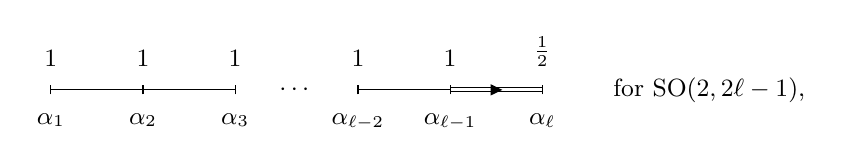
\begin{tikzpicture}[x=0.78cm,y=0.72cm,baseline=(current bounding box.center),font=\small]
\draw (0,0)--(3,0);
\node at (4,0) {$\cdots$};
\draw (5,0)--(6.5,0);
\draw[double distance=1.0pt] (6.5,0)--(8,0); \fill (7.35,0)--(7.16,0.10)--(7.16,-0.10)--cycle;
\foreach \x/\a/\v in {0/{\alpha_1}/1,1.5/{\alpha_2}/1,3/{\alpha_3}/1,5/{\alpha_{\ell-2}}/1,6.5/{\alpha_{\ell-1}}/1,8/{\alpha_\ell}/{\frac12}}{
  \draw (\x,-0.08)--(\x,0.08);
  \node[above=5pt] at (\x,0) {$\v$};
  \node[below=5pt] at (\x,0) {$\a$};
}
\node[anchor=west] at (9,0) {for $\SO(2,2\ell-1)$,};
\end{tikzpicture}
\]
\[
\begin{tikzpicture}[x=0.78cm,y=0.72cm,baseline=(current bounding box.center),font=\small]
\draw (0,0)--(3,0);
\node at (4,0) {$\cdots$};
\draw (5,0)--(6.5,0);
\draw (6.5,0)--(8,0.62);
\draw (6.5,0)--(8,-0.62);
\foreach \x/\a in {0/{\alpha_1},1.5/{\alpha_2},3/{\alpha_3},5/{\alpha_{\ell-3}},6.5/{\alpha_{\ell-2}}}{
  \draw (\x,-0.08)--(\x,0.08);
  \node[above=5pt] at (\x,0) {$1$};
  \node[below=5pt] at (\x,0) {$\a$};
}
\draw (8,0.54)--(8,0.70);
\draw (8,-0.70)--(8,-0.54);
\node[above=2pt] at (8,0.62) {$\frac12$};
\node[below=2pt] at (8,-0.62) {$\frac12$};
\node[anchor=west] at (8.55,0.62) {$\alpha_{\ell-1}$};
\node[anchor=west] at (8.55,-0.62) {$\alpha_\ell$};
\node[anchor=west] at (10.4,0) {for $\SO(2,2\ell-2)$.};
\end{tikzpicture}
\]
Let $w$ be a dominant weight of a spin or half-spin representation, and let $\sigma$ be the opposition involution. The point is that
\[
\langle w,r_0\rangle+\langle\sigma w,r_0\rangle=1.
\]

\section*{5. Construction of Families of Abelian Varieties}

We shall use the following theorem of A. Borel (to appear).

\paragraph{5.1. Theorem (A. Borel).} \emph{Let $X/\Gamma$ be the quotient of a Hermitian symmetric domain by a torsion-free arithmetic group. It is known [2] that $X/\Gamma$ is naturally a quasi-projective algebraic variety. Let $S$ be a reduced scheme over $\C$ and let $f:S^{\mathrm{an}}\to X/\Gamma$ be a morphism of analytic spaces. Then $f$ is algebraic.}

Let $S$ be smooth over $\C$. For the notion of a variation of Hodge structures $\underline H$ on $S$, and of a polarization of $\underline H$, we refer to Griffiths [6]. We write $\underline H_\Z$ for the local system of free $\Z$-modules on $S$ defined by $\underline H$, and $\underline H_s$ for the fiber Hodge structure of $\underline H$ at $s\in S$.

For $X$ the Siegel upper half-space, Theorem 5.1 has the following corollary, which generalizes 2.3.

\paragraph{5.2. Scholium.} \emph{The functor $(a:A\to S)\mapsto R^1a_*\Z$ identifies polarized abelian schemes $A$ over $S$ with polarized variations of Hodge structures of type $\{(0,1),(1,0)\}$ on $S$.}

\paragraph{5.3.} In the category of variations of Hodge structures on $S$, all the usual tensor operations make sense. Thus
\begin{enumerate}[label=\alph*)]
\item if $\underline H$ and $\underline H'$ are variations of Hodge structures, there are variations of Hodge structures
\[
\underline H\otimes\underline H',\qquad
\underline{\Hom}(\underline H,\underline H'),\qquad
\bigwedge\nolimits^n\underline H,\qquad
\underline H^\vee,\qquad
\underline{\End}(\underline H),\ldots.
\]
\end{enumerate}

\clearpage

\begin{enumerate}[label=\alph*),start=2]
\item if $\underline H$ is a variation of Hodge structures of weight $0$, and $\psi$ is a polarization of $\underline H$ (or any symmetric morphism of Hodge structures $\underline H\otimes\underline H\to\Z(0)$), then $C(\underline H,\psi)$ and $C^+(\underline H,\psi)$ are defined. At every point $t\in S$, with the notation of 3.4, one has
\[
C^+(\underline H,\psi)_t=C^+(\underline H_t,\psi)_{\ad}.
\]
\end{enumerate}

\paragraph{5.4.} Let $(V_\Z,B)$ be as in 4.1, and let $X$ be the set of $h:\underline S\to\SO(V_\R)$ of the type considered in 4.1. Giving such an $h$ is equivalent to giving a two-dimensional subspace $V^-_\R$ of $V_\R$, on which $B$ is negative definite, together with an orientation of $V^-_\R$: for $z=\tau\cdot e^{i\theta}\in\underline S(\R)=\C^*$, $h(z)$ induces the identity on the orthogonal complement of $V^-_\R$ and the rotation through angle $2\theta$ on $V^-_\R$. The group $\mathrm O(V_\R)$ acts on $X$ by transport of structure: $(g*h)(z)=g\cdot h(z)\cdot g^{-1}$, and the description above makes it geometrically evident that $X$ is a homogeneous space under $\SO(V_\R)$. The stabilizer of $h\in X$ is a subgroup $\SO(2)\times\SO(n)$, the identity component of a \emph{maximal} compact subgroup.

\paragraph{5.5.} For $h\in X$, let $F_h$ be the corresponding Hodge filtration of $V_\C$. The function $h\mapsto F_h^1$ identifies $X$ with an open subset of the space of isotropic lines in $V_\C$. This construction endows $X$ with a complex structure for which $F_h$ is a holomorphic function of $h$. It is known that, for this structure, the (two) connected components of $X$ are Hermitian symmetric domains.

\paragraph{5.6.} Let $W_\Q$ be a weight-$n$ representation of the algebraic group $\CSpin(V_\Q)$: $w(x)*y=x^n\cdot y$. Let $\underline W_\Q$ be the constant local system on $X$ with fiber $W_\Q$. The group $\CSpin(V_\Q)$ acts on $(X,\underline W_\Q)$ by
\[
\gamma*(w\text{ at }h\in X)=(\gamma w\text{ at }\gamma h\gamma^{-1}\in X).
\]
Each $h\in X$ defines $\tilde h:\underline S\to\CSpin(V_\R)$, hence a $\Q$-Hodge structure on the fiber of $\underline W_\Q$ at $h\in X$. Thus one obtains a variation of $\Q$-Hodge structures of weight $n$ on $X$, again denoted $\underline W_\Q$:
\begin{enumerate}[label=\alph*)]
\item the Hodge filtration is a holomorphic function of $h$;
\item the transversality axiom is satisfied (we shall use it only in a trivial case).
\end{enumerate}
This construction is compatible with tensor products. In particular, a polarization $\psi:W_\Q\otimes W_\Q\to\underline{\Q}(-n)$ of the representation $W_\Q$ defines a polarization of $\underline W_\Q$.

Let $W_\Z$ be an integral lattice in $W_\Q$ and let $\Gamma$ be a subgroup of $\CSpin(V_\Q)$, discrete in $\CSpin(V_\R)$, acting freely on $X$ and satisfying $\Gamma W_\Z=W_\Z$. Then the constant local system $\underline W_\Z$ on $X$, with fiber $W_\Z$, underlies a $\Gamma$-equivariant variation of Hodge structure $\underline W$ on $X$ as above. Passing to the quotient, it defines a variation of Hodge structures $\underline W$ on $X/\Gamma$.

\clearpage

If $W_\Q$ is a representation of $\SO(V_\Q)$, the same construction applies to discrete subgroups of $\SO(V_\Q)$.

\paragraph{5.7. Proposition.} \emph{Let $(\underline H,\psi)$ be a polarized variation of Hodge structures of type $\{(-1,1),(0,0),(1,-1)\}$, with $h^{1,-1}=1$, on a smooth connected scheme $S$. There exist}
\begin{enumerate}[label=\alph*)]
\item \emph{a finite surjective étale cover $u:S_1\to S$;}
\item \emph{an abelian scheme $A$ over $S_1$;}
\item \emph{a $\Z$-algebra $C$, and $\mu:C\hookrightarrow\End_{S_1}(A)$;}
\item \emph{an isomorphism of variations of Hodge structures}
\[
u:C^+(\underline H,\psi)\xrightarrow{\sim}\underline{\End}_C(R^1a_*\Z)
\]
\emph{which induces an isomorphism of local systems of algebras}
\[
u_\Z:C^+(\underline H_\Z,\psi)\xrightarrow{\sim}\underline{\End}_C(R^1a_*\Z).
\]
\end{enumerate}

Let $(V_\Z,B)$ be a $\Z$-module equipped with a symmetric bilinear form, isomorphic to $(H_{s\Z},\psi)$, and retain the notation of 5.4. Let $n$ be an integer,
\[
\Gamma=\{\gamma\in\SO(V_\Z)\mid\gamma\equiv1\pmod n\}
\]
and
\[
\widetilde\Gamma=\{\gamma\in\CSpin(V_\Q)\mid\alpha(\gamma)\equiv1\pmod n\text{ in }C^+(V_\Z)\}.
\]
Assume $n$ is large enough that $\Gamma$ and $\widetilde\Gamma$ are torsion-free.

There is a finite étale cover $v:S'_1\to S$ such that the local system $v^*\underline H_{\Z/n\Z}$ is trivial. Choose an isomorphism $\sigma_n$ between this local system and the constant local system $\underline V_{\Z/n\Z}$. Let $s\in S'_1$ and let $\sigma:V_\Z\xrightarrow{\sim}H_{s\Z}$ be an isometry such that $\sigma\equiv\sigma_n\pmod n$ (we choose $\sigma_n$ so that such $\sigma$ exist). The Hodge structure $h_s$ on $H_s$ defines $\sigma^{-1}(h_s)\in X$. The image of $\sigma^{-1}(h_s)$ in $X/\Gamma$ depends only on $s$. We thus define
\[
m:S'_1\longrightarrow X/\Gamma
\]
and an isomorphism compatible with the polarizations
\[
\underline H\simeq m^*\underline V.
\]
Let
\[
S_1=S'_1\times_{X/\Gamma}X/\widetilde\Gamma:
\]
\begin{center}
\begin{tikzpicture}[x=1.05cm,y=0.9cm,baseline=(current bounding box.center)]
\node (Sone) at (0,2.0) {$S_1$};
\node (Sp) at (-2.1,0.75) {$S'_1$};
\node (Xt) at (2.1,0.75) {$X/\widetilde\Gamma$.};
\node (Xg) at (0,-0.9) {$X/\Gamma$};
\node (S) at (-4.1,0.75) {$S$};
\draw[->] (Sone)--node[above left] {$p_1$} (Sp);
\draw[->] (Sone)--node[above right] {$p_2$} (Xt);
\draw[->] (Sp)--node[above] {$v$} (S);
\draw[->] (Sp)--node[below left] {$m$} (Xg);
\draw[->] (Xt)--(Xg);
\end{tikzpicture}
\end{center}

\clearpage

On $S_1$, one has
\begin{enumerate}[label=\alph*)]
\item an isomorphism $(v p_1)^*H\simeq(m p_1)^*\underline V$;
\item a variation of Hodge structure, the pullback by $p_2$ of the one on $X/\widetilde\Gamma$ defined by the representation $(C^+(V_\Q))_s$ and the lattice $C^+(V_\Z)$.
\end{enumerate}
By 5.2, 5.6 and 4.5, this variation of Hodge structures corresponds to an abelian scheme $a:A\to S_1$.

c) Let $C$ be the algebra $C^+(V_\Z)$. The abelian scheme constructed in b) has complex multiplication by $C$, and the variation of Hodge structures $\underline{\End}_C(R^1a_*\Z)$ is
\[
p_2^*((\underline C^+(V_\Z))_{\ad}).
\]
Combining this with a), one obtains an isomorphism of local systems of algebras and of variations of Hodge structures
\[
\underline C^+(v p_1^*H)\simeq\underline{\End}_C(R^1a_*\Z).
\]
This proves 5.7.

\section*{6. $K3$ Surfaces}

\paragraph{6.1.} A polarized $K3$ surface over a field $K$ of characteristic $0$ is a $K3$ surface over $K$, say $Y$, endowed with an element $\eta\in\NS(Y)=\Pic(Y)$ which is the class of an ample invertible sheaf. For $K=\C$, we shall identify $\NS(Y)$ with a subset of $H^2(Y,\Z)$.

\paragraph{6.2.} A \emph{family of $K3$ surfaces} parametrized by a scheme $S$ of characteristic $0$ is a proper flat morphism $f:Y\to S$ whose fibers are $K3$ surfaces. A \emph{polarization} of $f:Y\to S$ is a section $\eta$ of $\Pic_S(Y)$ which, for every $s\in S$, is a polarization of $Y_s=f^{-1}(s)$.

For every prime number $\ell$, we identify $\eta$ with a section of $R^2f_*\Z_\ell$; we denote by $P^2f_*\Z_\ell$ the orthogonal complement of $\eta$ (for the cup product); it is a subsheaf of $R^2f_*\Z_\ell$ in $\Z_\ell$-modules. The cup product
\[
R^2f_*\Z_\ell\otimes R^2f_*\Z_\ell\longrightarrow R^4f_*\Z_\ell
\]
and the trace morphism
\[
R^4f_*\Z_\ell\xrightarrow{\sim}\underline{\Z}_\ell(-2)
\]
induce
\[
\tag{6.2.1}
\psi_\ell:P^2f_*\Z_\ell(1)\otimes P^2f_*\Z_\ell(1)\longrightarrow\underline{\Z}_\ell.
\]

\paragraph{6.3.} Take $S$ to be a scheme of finite type over $\C$. Then $R^2f_*\Z$ is a variation of Hodge structures on $S$; $\eta$ is everywhere of type $(1,1)$ and its orthogonal complement $P^2f_*\Z$ is again a variation of Hodge structures. As above, the cup product defines
\[
\tag{6.3.1}
\psi:P^2f_*\Z(1)\otimes P^2f_*\Z(1)\longrightarrow\underline{\Z}.
\]

\clearpage

This time, the negative of $\psi$ is a polarization of the variation of Hodge structures $P^2f_*\Z(1)$. Moreover, $\psi_\ell$ is obtained from $\psi$ via the isomorphism
\[
(P^2f_*\Z(1)_\Z)\otimes\Z_\ell\simeq P^2f_*\Z_\ell(1).
\]
For every $s\in S$, the fiber at $s$, $(P^2f_*\Z(1))_s$, is the primitive part of the cohomology $H^2(Y_s,\Z)$. The Hodge structure on $(P^2f_*\Z(1))_s$ is of type $\{(-1,1),(0,0),(1,-1)\}$, with $h^{-1,1}=1$ ((1.1)(i)).

The action of $\pi_1(S,s)$ on $H^2(Y_s,\Z)$ induces
\[
\tag{6.3.2}
\pi:\pi_1(S,s)\longrightarrow \mathrm O(P^2(Y_s,\Z)(1)_\Z,\psi).
\]

\paragraph{6.4. Proposition.} \emph{For every complex polarized $K3$ surface $Y_0$, there exists a family of polarized $K3$ surfaces $f:Y\to S$ as above, with $Y_s\simeq Y_0$ for some $s\in S$, such that the image of $\pi$ in (6.3.2) has finite index.}

Let $f_T^\wedge:Y_T^\wedge\to T^\wedge$ be the versal formal deformation of $Y_0$. Since $H^0(Y_0,T^1)=0$, $T^\wedge$ is even a formal moduli scheme for $Y_0$, but this is immaterial. Since $H^2(Y_0,T^1)=0$ ((1.1)(i)), $T^\wedge$ is the spectrum of a formal power-series ring over $\C$. From $f_T^\wedge$ one obtains a (non-polarized) variation of Hodge structures on $T^\wedge$. By (1.1.1), this is the universal deformation of \{the Hodge structure $H^2(Y_0,\Z)$, endowed with the cup product\}.

Let $\bar\eta$ be the image of $\eta$ under the composite map
\[
H^2(Y_0,\Z)\longrightarrow H^2_{\mathrm{DR}}(Y_T^\wedge/T^\wedge)
\longrightarrow R^2f_{T*}^\wedge\mathcal O.
\]
Let $S^\wedge$ be the formal subscheme of $T^\wedge$ with equation $\bar\eta=0$, and let $f^\wedge:Y^\wedge\to S^\wedge$ be induced by $f_T^\wedge$. Since $h^{0,2}=1$, $S^\wedge\subset T^\wedge$ is defined by one equation; this equation is part of a regular system of parameters, so $S^\wedge$ is a power-series ring. On $S^\wedge$, $\eta$ comes from an ample invertible sheaf $\mathcal O(1)$ on $Y^\wedge$; hence $f^\wedge$ is algebraizable. Moreover, on $S^\wedge$, the polarized variation of Hodge structure $(P^2(Y^\wedge/S^\wedge,\Z)(1),\psi)$ is a universal deformation of $(P^2(Y_0,\Z)(1),\psi)$.

Put $S^\wedge=\Spec(A^\wedge)$, and express $A^\wedge$ as an inductive limit of rings of finite type over $\C$. Since $Y^\wedge$ is algebraizable, there is a Cartesian diagram
\[
\begin{tikzcd}[column sep=2.4em,row sep=2.2em]
Y^\wedge \arrow[r] \arrow[d,"f^\wedge"] & Y \arrow[d,"f"]\\
S^\wedge \arrow[r] & S
\end{tikzcd}
\]
with $S$ of finite type over $\C$ and $Y$ a polarized family of $K3$ surfaces over $S$ (we do not assume that $S^\wedge$ is a completion of $S$). We may take $S$ normal and connected; let $s\in S$ be the image of the closed point of $S^\wedge$.

\clearpage

In fact, by Artin's approximation theorem [1], one can find $S$ such that $S^\wedge$ is a completion of $S$. Then $S$ is smooth in a neighborhood of $s$. The simplifications resulting from such a choice are mostly psychological.

Let us show that $f:Y\to S$ satisfies 6.2. After replacing $S$ by a finite étale cover, one defines, as in 5.7, a holomorphic map
\[
m:S\longrightarrow X/\Gamma
\]
from $S$ to a moduli space of polarized Hodge structures such that the inverse image of the universal family of Hodge structures on $X/\Gamma$ is $(P^2(Y/S,\Z)(1),\psi)$.

By Borel (5.1), $m$ is a morphism of schemes. The morphism $m$ is dominant, since the composite $m^\wedge:S^\wedge\to X/\Gamma$ is dominant. It follows (see, for example, P. Deligne, Théorie de Hodge II. Publ. Math. IHES 40, Lemma 4.4.17) that $m(\pi_1(S,s))$ has finite index in $\pi_1(X/\Gamma,m(s))=\Gamma$, which itself has finite index in the orthogonal group.

\paragraph{6.5. Proposition.} \emph{Let $Y_0$ be a polarized $K3$ surface over a field $K$ of characteristic $0$. There exist:}
\begin{enumerate}[label=\alph*)]
\item \emph{a scheme $S$ of finite type over $\Q$, and a family $f:Y\to S$ of polarized $K3$ surfaces, parametrized by $S$;}
\item \emph{a finite extension $K'$ of $K$ and $v:\Spec(K')\to S$ such that $v^*Y$ is isomorphic to $Y_0\otimes_K K'$;}
\item \emph{an abelian scheme $a:A\to S$ over $S$;}
\item \emph{a $\Z$-algebra $C$ and $\mu:C\to\End_S(A)$;}
\item \emph{an isomorphism of sheaves of $\Z_\ell$-algebras on $S$}
\[
u:C^+(P^2f_*\Z_\ell(1),\psi_\ell)\iso \underline{\End}_C(R^1a_*\Z_\ell).
\]
\end{enumerate}

We reduce to the case where $K$ is of finite type over $\Q$. Choose a complex embedding $\sigma:K\to\C$ and apply 6.4 to $Y_0\otimes_K\C$ to obtain a family of polarized $K3$ surfaces $f_1:Y_1\to S_1$. Apply 5.7 to $f_1$; one obtains a family $f_2:Y_2\to S_2$ still satisfying the conclusion of 6.4, and, over $S_2$, an abelian scheme $a_2:A_2\to S_2$ with complex multiplication $\mu_2:C\to\End_{S_2}(A_2)$ and an isomorphism
\[
u_2:C^+(P^2f_{2*}\Z(1),\psi)\iso \underline{\End}_C(R^1a_{2*}\Z)
\]
of local systems of algebras. The system of complex schemes and morphisms
\[
\overline E_2=(S_2,f_2,Y_2,a_2,A_2,\mu_2)
\]
is defined by finitely many equations. Hence there exists an extension $K_3$ of $K$ of finite type, with $K\subset K_3\subset\C$, and, over $K_3$, a system
\[
\overline E_3=(S_3;f_3,Y_3,a_3,A_3,\mu_3)
\]
which, after extension of scalars from $K_3$ to $\C$, gives $\overline E_2$.

\clearpage

\paragraph{6.5.1. Lemma.} \emph{There exists a unique isomorphism of sheaves of $\Z_\ell$-algebras}
\[
u_3:C^+(P^2f_{3*}\Z_\ell(1),\psi_\ell)\iso
\underline{\End}_C(R^1a_{3*}\Z_\ell).
\]
It is enough to verify that such an isomorphism exists and is unique after extending scalars to an algebraic closure of $K_3$, for example $\C$. Existence holds by construction, and uniqueness follows from 3.5. Indeed, for $s\in S_2$, the image of $\pi_1(S_2,s)$ in $\mathrm O(P^2(Y_{2s},\Z),\psi)$ has finite index and therefore contains a Zariski-dense subgroup of $\mathrm{SO}$.

Let $T$ be an integral scheme of finite type over $\Q$, with function field $K_3$. For a suitable $T$, $\overline E_3$ is the generic fiber of a system $\overline E=(S,f,Y,a,A,\mu)$ over $T$, and $u_3$ extends to
\[
u:C^+(P^2f_*\Z_\ell(1),\psi_\ell)\iso
\underline{\End}_C(R^1a_*\Z_\ell).
\]
The existence of $K'$ as in b) is easily verified, and this completes the proof.

\paragraph{6.6.} We prove Theorem 1.3. Let $f_V:Y_V\to\Spec(V)$ be as in 1.2(i). Let $K$ be the fraction field of $V$, and apply 6.5 to the surface $Y_K=Y\otimes_V K$ over $K$, endowed with any polarization. After replacing $V$ by its normalization in a finite extension of $K$, one may suppose that there exists $\overline E=(S,f,Y,a,A,\mu,u)$ as in 6.5, such that $Y_K$ is the inverse image of $Y$ under $v:\Spec(K)\to S$. Taking the inverse image gives an abelian variety with complex multiplication $(A_K,\mu)$ over $K$.

Let $\overline K$ be an algebraic closure of $K$, and let $\overline k$ be the corresponding algebraic closure of $k$ (the residue field of the normalization of $V$ in $\overline K$). From $u$ one obtains an isomorphism of $\Gal(\overline K/K)$-modules
\[
\tag{6.6.1}
C^+(P^2(Y_{\overline K},\Z_\ell)(1),\psi_\ell)\iso
\End_C(H^1(A_{\overline K},\Z_\ell)).
\]
Since $Y_V$ is smooth over $V$, the inertia group $I$ acts trivially on
\[
H^2(Y_{\overline K},\Z_\ell)\simeq H^2(Y_{\overline k},\Z_\ell).
\]
The polarization defines an invariant $\eta$ in $H^2(Y_{\overline k},\Z_\ell)(1)$, whose orthogonal complement is $P^2(Y_{\overline k},\Z_\ell)(1)$, and $I$ acts trivially on
\[
C^+(P^2(Y_{\overline K},\Z_\ell)(1),\psi_\ell)\simeq
C^+(P^2(Y_{\overline k},\Z_\ell)(1),\psi_\ell).
\]
Since $I$ acts trivially on $\End_C(H^1(A_{\overline K},\Z_\ell))$ and commutes with the complex multiplication, it acts through the center of $C\otimes\Q_\ell$. It is also known that a subgroup of finite index in $I$ acts unipotently on $H^1(A_{\overline K},\Z_\ell)$; it follows that $I$ acts through one of its finite quotients. After a further finite extension of $K$, one may therefore suppose that $A_K$ has good reduction over $V$.

For $A_{\overline k}$, the special fiber of its reduction, (6.6.1) reduces to an isomorphism of $\Gal(\overline k/k)$-modules
\[
\tag{6.6.2}
C^+(P^2(Y_{\overline k},\Z_\ell)(1),\psi_\ell)\iso
\End_C(H^1(A_{\overline k},\Z_\ell)).
\]

\clearpage

By Weil's theory for $A_k$, the eigenvalues of Frobenius acting on $C^+(P^2(Y_{\overline k},\Z_\ell)(1),\psi_\ell)$ are algebraic numbers all of whose complex conjugates have absolute value $1$. We have
\[
\mathop{\bigwedge}\limits^2(P^2(Y_{\overline k},\Z_\ell)(1))
\subset C^+(P^2(Y_{\overline k},\Z_\ell)(1),\psi_\ell),
\]
and, since $\dim P^2(Y_{\overline k},\Z_\ell)>2$ (as is the case here), it follows that the eigenvalues of Frobenius acting on $P^2(Y_{\overline k},\Z_\ell)(1)$ likewise have complex absolute value $1$. The same assertion holds for $H^2(Y_{\overline k},\Z_\ell)(1)$, and the theorem follows.

\section*{7. Remarks}

\paragraph{7.1.} Let $H$ be a rational Hodge structure. We shall call the \emph{Mumford--Tate group} of $H$ the smallest algebraic subgroup $G$ of $\GL(H_\Q)$, defined over $\Q$, such that $G(\R)$ contains the image of $h:\underline S\to\GL(H_\R)$. For polarizable $H$, $G$ is reductive. This definition differs from Mumford's: if $H$ has weight $n\ne0$, our $G$ contains the scalar homotheties. By 2.9, every homogeneous representation of $G$ carries a natural Hodge structure.

One of the key points in the proof of 1.3 was that the Hodge structure $H^2(X,\Q)$, for $X$ a $K3$ surface, ``is expressible'' in terms of abelian varieties, in the following sense.

\paragraph{7.2. Definition.} A rational Hodge structure $H$ is expressible in terms of abelian varieties if it belongs to the smallest category of rational Hodge structures stable under direct factors, direct sums, and tensor products, and containing the $H^1(A,\Q)$ for $A$ an abelian variety, as well as the $\Q(n)$.

In this paper, we show that this property of $K3$ surfaces is exceptional.

Consider the following property of a rational Hodge structure with Mumford--Tate group $G$.
\begin{quote}
\raggedright\noindent $(*)$\quad The Hodge structure on the adjoint representation $\Lie(G)$ of $G$ is purely of type $\{(-1,1),(0,0),(1,-1)\}$.
\end{quote}

\paragraph{7.3. Proposition.} \emph{If a rational Hodge structure $H$ is expressible in terms of abelian varieties, then condition $(*)$ holds.}

Indeed,
\begin{enumerate}[label=(\alph*)]
\item the Hodge structures $H^1(A,\Q)$ and $\Q(n)$ satisfy $(*)$;
\item condition $(*)$ is stable under direct factors, direct sums, and tensor products.
\end{enumerate}

\clearpage

\paragraph{7.4.} Analogous arguments show that if $H$ is expressible in terms of abelian varieties, then the reductive group $G_\C$ has no ``factors'' of exceptional type.

\paragraph{7.5. Proposition.} \emph{Let $\underline H$ be a polarized variation of Hodge structures on an irreducible scheme $S$. For $s\in S$ outside a meagre subset of $S$, there exists a finite-index subgroup of $\pi_1(S,s)$ whose image in $\GL(H_{s\Z})$ is contained in the Mumford--Tate group of $H_s$.}

At every point of $S$, the Mumford--Tate group $G_s$ of $H_s$ may be described as follows. It is the algebraic subgroup of $\GL(H_{s\Q})$ that fixes all tensors $t\in H_{s\Q}^{\otimes n}\otimes H_{s\Q}^{*\otimes n}$ $(n>0)$ that are rational of type $(0,0)$. From this description it follows readily that, outside a meagre subset $M$ of $S$, $G_s$ is locally constant: for $s\notin M$, the largest subspace of type $(0,0)$, $V(n)_s\subset H_{s\Q}^{\otimes n}\otimes H_{s\Q}^{*\otimes n}$, is locally constant and defines a local system $V(n)$ on $S$. This local system underlies a polarized variation of Hodge structures of type $(0,0)$; hence $V(n)_s$ carries a positive-definite quadratic form invariant under $\pi_1(S,s)$, and $\pi_1(S,s)$ acts on $V(n)_s$ through a finite group. One concludes by noting that there is a finite sequence of integers $n_i$ such that $G_s$ is the algebraic subgroup of $\GL(H_{s\Q})$ acting trivially on the $V(n_i)_s$.

\paragraph{7.6.} Consider a Lefschetz pencil of hypersurfaces of degree $d$ and odd dimension $2r-1$.
\[
\begin{tikzcd}[column sep=4.2em,row sep=2.6em]
X \arrow[r,hook] \arrow[d,"f"'] & \mathbb P^{2r}(\C)\times\mathbb P^1(\C) \arrow[dl,"pr_2"]\\
\mathbb P^1(\C). &
\end{tikzcd}
\]
Let $U\subset\mathbb P^1(\C)$ be the complement of the finite set of $t\in\mathbb P^1(\C)$ for which the hypersurface $X_t=f^{-1}(t)$ is singular, and let $s\in U$. The cup product is an alternating form $\psi$ on $H^{2r-1}(X_s,\Z)$, preserved by monodromy, whence
\[
m:\pi_1(U,s)\longrightarrow \operatorname{Sp}(H^{2r-1}(X_s,\Z),\psi).
\]
By a theorem of Kajdan and Margulis, the image of $m$ is Zariski-dense in the symplectic group. By 7.5, for $s$ outside a meagre (in fact, countable) subset of $\mathbb P^1(\C)$, the Mumford--Tate group of the rational Hodge structure $H^{2r-1}(X_s,\Q)$ is therefore the entire group of symplectic similitudes. If this Hodge structure is not of Hodge level at most one (i.e. if some $h^{pq}$ with $|q-p|\ne1$ is nonzero), it follows from 7.3 that it is not expressible in terms of abelian varieties.

\clearpage

\begin{center}
\bfseries Bibliography
\end{center}
\begin{enumerate}[label=\arabic*.]
\item Artin, M.: Algebraisation of formal moduli I. Global analysis. Papers in honor of K. Kodaira. Princeton University Press.
\item Baily, W.~L., Borel, A.: Compactification of arithmetic quotients of bounded symmetric domains. Annals of Math. (2) \textbf{84}, 442--528 (1966). (MR 35, 6870).
\item Bourbaki, N.: Algèbre -- Chapitre 9. Paris: Hermann 1959. Act. Sci. et Ind. 1272.
\item Deligne, P.: Travaux de Griffiths -- Séminaire Bourbaki 376 -- mai 1970. Lecture Notes in mathematics 180. Berlin-Heidelberg-New York: Springer 1971.
\item Demazure, M.: Motifs des variétés algébriques -- Séminaire Bourbaki 365 -- mai 1970. Lecture Notes in mathematics 180. Berlin-Heidelberg-New York: Springer 1971.
\item Griffiths, P.~A.: Periods of integrals on algebraic manifolds. (Summary of main results and discussions of open problems and conjectures.) Bull. Am. Math. Soc. \textbf{75}, 228--296 (1970).
\item Kuga, M., Satake, I.: Abelian varieties attached to polarized K3-surfaces. Math. Ann. \textbf{169}, 239--242 (1967). (MR 35 1602).
\item \v{S}afarevitch, Chafonevitch, I.~R., Averbuch, B.~C., Va\"inberg, Ju.~R., Jujtchenko, A.~B., Manin, Ju.~I., Moishezon, B.~C., Tjurina, C.~I., Tjurin, A.~I.: Algebraic surfaces. Trudi Mat. Inst. Steklov LXXV.
\item Weil, A.: Variétés abéliennes et courbes algébriques. Paris: Hermann 1948.
\end{enumerate}

\begin{flushright}
Pierre Deligne\\
Institut des Hautes Études Scientifiques\\
35, Route de Chartres\\
F-91 Bures-sur-Yvette\\
France
\end{flushright}

\begin{center}
\emph{(Received 6 August 1971/1 October 1971)}
\end{center}

\end{document}
